\documentclass{beamer}
\usepackage[italian]{babel}
\usepackage[utf8]{inputenc}
\usepackage[T1]{fontenc}
\title{prove tecniche di fallimento...}
\author{Giorgio Barone}
\date{Matino, \today}
\institute[]{Matino è una città del Salento!}
\logo{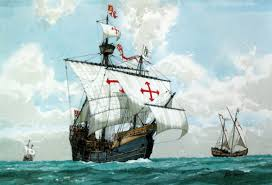
\includegraphics[width=15mm]{nave_logo.jpeg}}
\usetheme{Berkeley}

\usecolortheme{default}
\setbeamercovered{dynamic}
\theoremstyle{definition}
\newtheorem{definizione}{Definizione}
\theoremstyle{plain}
\newtheorem{property}{Proprietà}
\theoremstyle{plain}
\newtheorem{teorema}{Teorema}

% pacchetti 
\usepackage{mathtools} % qui per i delimitatori matematici
\usepackage{amsmath} %per simboli matematici e le formule allineate (ambiente             split)
\usepackage[output-decimal-marker={,}]{siunitx} % per le unità di misura nel SI
\usepackage{amssymb} %per simboli matematici 
\usepackage{wrapfig} % per scrivere accanto alle figure e non solo in alto e in basso
%fine pacchetti
 
% comandi personalizzati
\DeclarePairedDelimiter{\abs}{\lvert}{\rvert}% valore assoluto o modulo
\DeclareUnicodeCharacter{2212}{-}
\newcommand{\Def}{\overset{\mathit{def}}{=}} %uguale per definizione

\newenvironment{system}%
{\left\lbrace\begin{array}{@{}l@{}}}%
    {\end{array}\right.}
% fine comandi personalizzati



\begin{document}

\begin{frame}
\maketitle
\end{frame}

\begin{frame}
\frametitle{La Cinematica e generalità sul moto}
La \emph{Cinematica} è la branca della Fisica che si occupa di descrivere il moto delle particelle e dei corpi senza entrare nel dettaglio sulla natura delle \emph{forze} o \emph{interazioni} che ne sono la causa.
Il termine "Cinematica" deriva dal greco antico "$ \kappa     \iota \nu \eta \mu \alpha $" che significa "movimento"

Per descrivere il moto di un oggetto di dimensioni macroscopiche, occorre tenere presente anche della geometria nello spazio che il corpo assume nel tempo. Si possono avere in generale tre tipi di moto: 

\begin{itemize}
\item traslazione ;
\item rotazione;
\item deformazione, quando viene modificata la geometria propria del corpo.
\end{itemize} 

\end{frame}

\begin{frame}

\frametitle{Un po' di definizioni \dots}

\begin{wrapfloat}{figure}{I}{0pt}
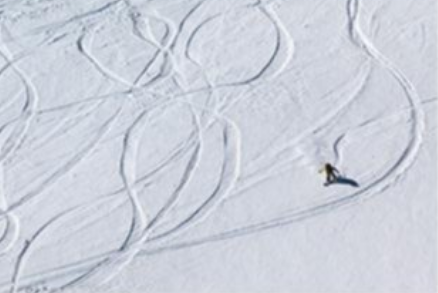
\includegraphics[width=0.4\columnwidth]{traiettoria.png}
\end{wrapfloat}

Il \emph{punto materiale} è un'approssimazione che si usa nei sistemi fisici quando ci si vuole occupare solo della traslazione nello spazio del corpo in movimento. Quasi sempre inoltre si assume come coincidente con il \emph{centro di massa} del corpo, cioè un punto in cui è concentrata tutta sua massa. 
\begin{definizione}
La successione nello spazio al passare del tempo dei punti materiali di un corpo è detta
 \emph{traiettoria} 
\end{definizione}

\end{frame}

\begin{frame}
\frametitle{Il moto è relativo!}

\begin{wrapfloat}{figure}{I}{0pt}
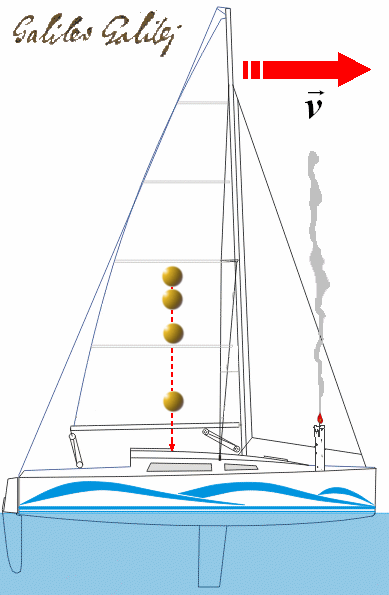
\includegraphics[width=0.4\columnwidth]{barca_galileo.png}
\end{wrapfloat}


Bisogna tener presente che il moto di qualunque oggetto materiale va riferito ad un \emph{sistema di riferimento}. Infatti potremmo chiederci se il moto di una palla lanciata in aria su di una barca in movimento appaia rettilineo verticale oppure parabolico: dipende dal sistema di riferimento dell'osservatore. Se esso è solidale con la barca è rettilineo verticale, se esso vede la barca muoversi dalla terraferma invece no. 

Fu Galileo il primo a definire questo concetto con chiarezza ed è a lui che dobbiamo il primo principio di \emph{Relatività}.

\end{frame}

\begin{frame}
\frametitle{Le Grandezze Fisiche nel Moto}
Affinché il moto sia quantificabile, occorre poter fare delle misure di grandezze fisiche. 
Una misura dello \emph{spazio} percorso è la distanza tra un punto materiale e l'origine del sistema di riferimento.
Abbiamo anche parlato di \emph{tempo} entro cui un punto materiale percorre una certa traiettoria. 
Perciò le prime due grandezze fondamentali che coinvolgono il moto sono \emph{lunghezza} e \emph{tempo}. 
Nel Sistema Internazionale di Misura (SI) la prima viene misurata in metri ($m$) o nei suoi multipli e sottomultipli decimali. Il tempo viene misurato in secondi ($s$), anche se i multipli comuni, i minuti e le ore, non fanno parte propriamente del SI perché sono multipli sessagesimali e non decimali.

\end{frame}


\begin{frame}
\frametitle{Lo spostamento}

\begin{wrapfloat}{figure}{I}{0pt}
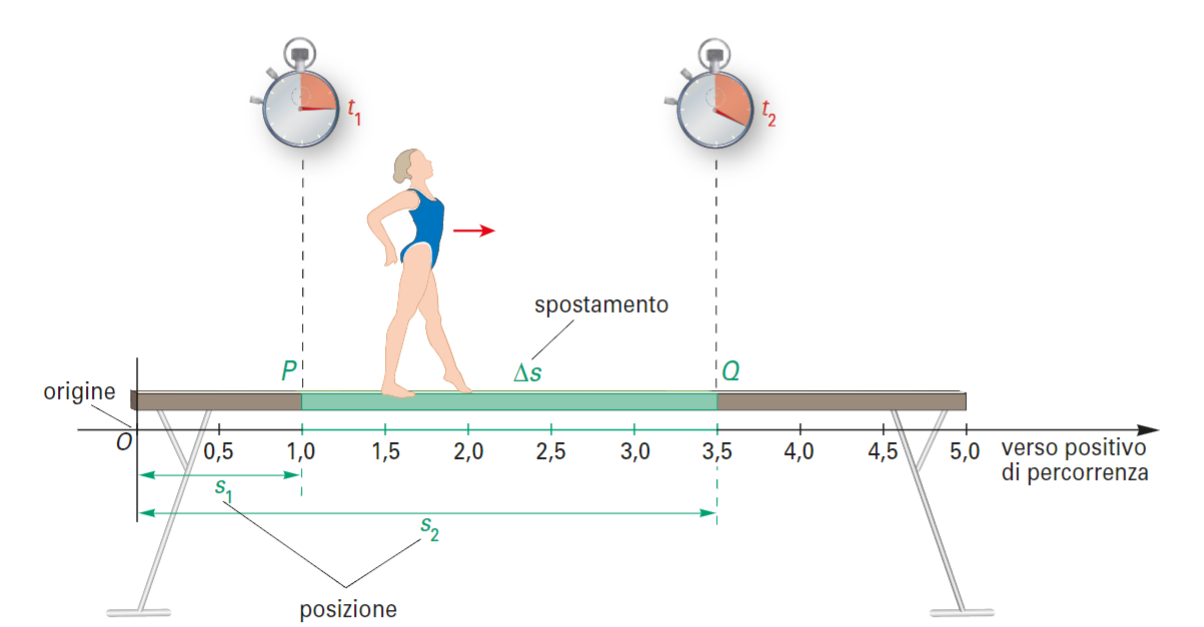
\includegraphics[width=0.6\columnwidth]{ginnasta_spostamento.png}
\end{wrapfloat}

Nella pratica, dovendo fare delle misure quantitative, riferiamo la \emph{posizione} di un punto materiale all'origine di una retta orientata.
$s_1$ rappresenta la posizione al tempo $t_1$ ed $s_2$ rappresenta la posizione al tempo $t_2$. 

\begin{definizione} 
Definiamo lo \emph{spostamento} $\Delta s$ come la differenza tra la posizione finale meno quella iniziale:
$\Delta s = s_f - s_i$
\end{definizione}

\end{frame}


\begin{frame}
\frametitle{Posizioni e spostamento come vettori}

La lettera greca $\Delta$ ("delta" maiuscola) posta prima di una grandezza fisica ne denota una variazione da uno stato iniziale ad uno finale.

\begin{wrapfloat}{figure}{I}{0pt}
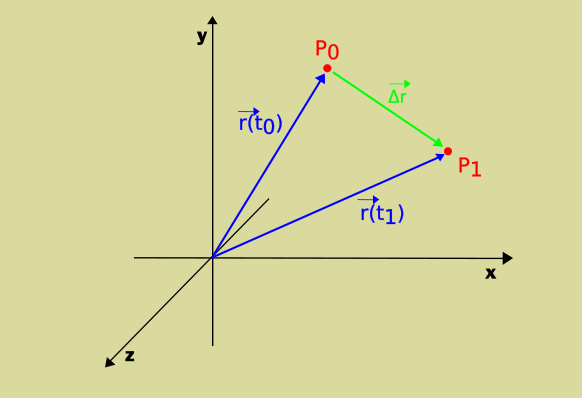
\includegraphics[width=0.6\columnwidth]{vettori_spostamento.png}
\end{wrapfloat}
NOTA: I punti materiali in genere sono situati nello spazio consono a 3 dimensioni, quindi nella forma più generale le posizioni e lo spostamento sono definibili come vettori nello spazio. La differenza tra vettori è quel vettore che collega le due punte e ha la punta coincidente con il "vettore sottraendo".

\end{frame}

\begin{frame}
\frametitle{La velocità}

\begin{definizione}
Si definisce velocità media il rapporto tra lo spostamento e l'intervallo di tempo entro cui è avvenuto: \newline
$ v_m = \frac{\Delta s}{\Delta t} = 
\frac{s_f - s_i}{t_f - t_i}$
\end{definizione}
\begin{wrapfloat}{figure}{I}{0pt}
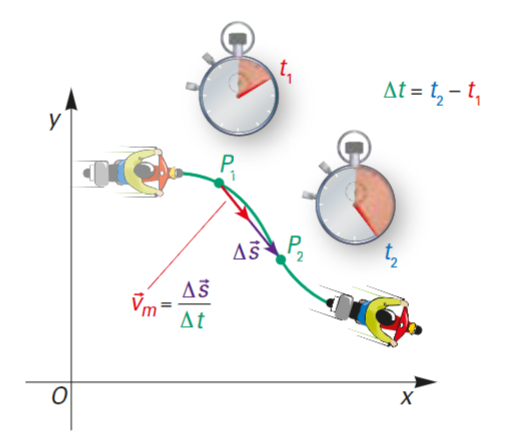
\includegraphics[width=0.4\columnwidth]{velocità_vettoriale.png}
\end{wrapfloat}

NOTA: Se lo spostamento viene considerato come uno scalare, allora anche la velocità è una grandezza scalare, perché corrisponde alla divisione per un intervallo di tempo che senz'altro è uno scalare. Ma se lo spostamento viene considerato come vettore, allora anche la velocità è  un vettore e conserva la direzione del vettore spostamento.

\end{frame}


\begin{frame}
\frametitle{Da chilometri orari a metri al secondo e viceversa}
Nel SI la velocità si misura in $m/s$, mentre comunemente può essere misurata anche, per esempio in $km/h$. La conversione è molto facile da fare: 
\[
1 \frac{km}{h} = \frac{10^3 m}{3600 s} = \frac{1}{3.6} \frac{m}{s}
\]

\[
1 \frac{m}{s} = \frac{10^{-3} km}{(1/3600) h} = \frac{3600}{1000} \frac{km}{h} = 3.6 \frac{km}{h}
\]

NOTA: Se nei calcoli si conservano le unità di misura correttamente, e si semplificano anche trattandole a tutti gli effetti come dei monomi in matematica, allora alla fine si avrà automaticamente anche una cosiddetta \emph{analisi dimensionale} già fatta!
\end{frame}


\begin{frame}
\frametitle{Il grafico spazio-tempo}

\begin{wrapfloat}{figure}{I}{0pt}
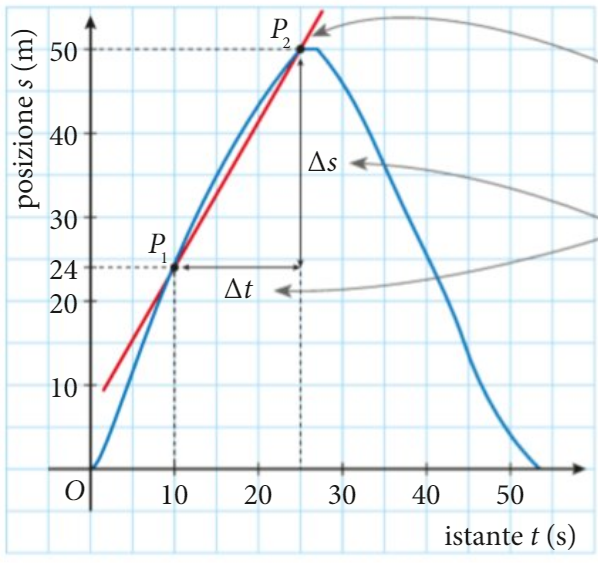
\includegraphics[width=0.5\columnwidth]{grafico_spazio_tempo.png}
\end{wrapfloat}

Un diagramma cartesiano dove nell'asse delle $x$ vi è il tempo, che è la variabile indipendente, e nell'asse delle $y$ vi è lo spazio, inteso come spostamento rispetto all'origine, nel moto unidimensionale, è detto \emph{grafico spazio-tempo}
Esso rappresenta graficamente la \emph{legge oraria del moto} cioè una \emph{funzione} dello spazio rispetto al tempo.


Si può vedere che presi due punti $P_1$ e $P_2$ sulla curva del grafico, la velocità media è la \emph{pendenza} della secante che congiunge i due punti di coordinate $(t_1, s_1)$ e 
$(t_2, s_2)$.

\end{frame}

\begin{frame}
\frametitle{La velocità istantanea}

\begin{wrapfloat}{figure}{I}{0pt}
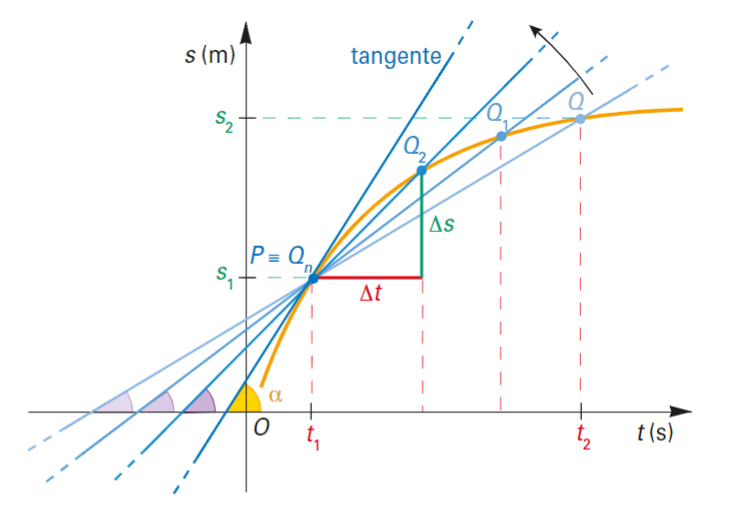
\includegraphics[width=0.5\columnwidth]{velocità_istantanea.png}
\end{wrapfloat}

Se prendiamo due punti sul grafico spazio-tempo sempre più vicini, cioè distanti intervalli di tempo, e quindi di spazio percorso, sempre più piccoli, la pendenza della secante approssimerà sempre meglio quella della tangente al grafico. 
La quantità fisica che corrisponde alla pendenza della tangente al grafico nel punto P è la \emph{velocità istantanea} in quel punto. Per chi conosce limiti e derivate, la velocità istantanea è per definizione la derivata dello spazio rispetto al tempo nel punto P.
\[
v = \lim\limits_{\Delta t \to 0} \frac{\Delta s}{\Delta t} \Def \frac{ds}{dt}
\]

\end{frame}


\begin{frame}
\frametitle{Il moto rettilineo uniforme}


\begin{definizione}
Un punto materiale si muove con \emph{moto rettilineo uniforme} quando percorre una traiettoria rettilinea con velocità costante.
\end{definizione}

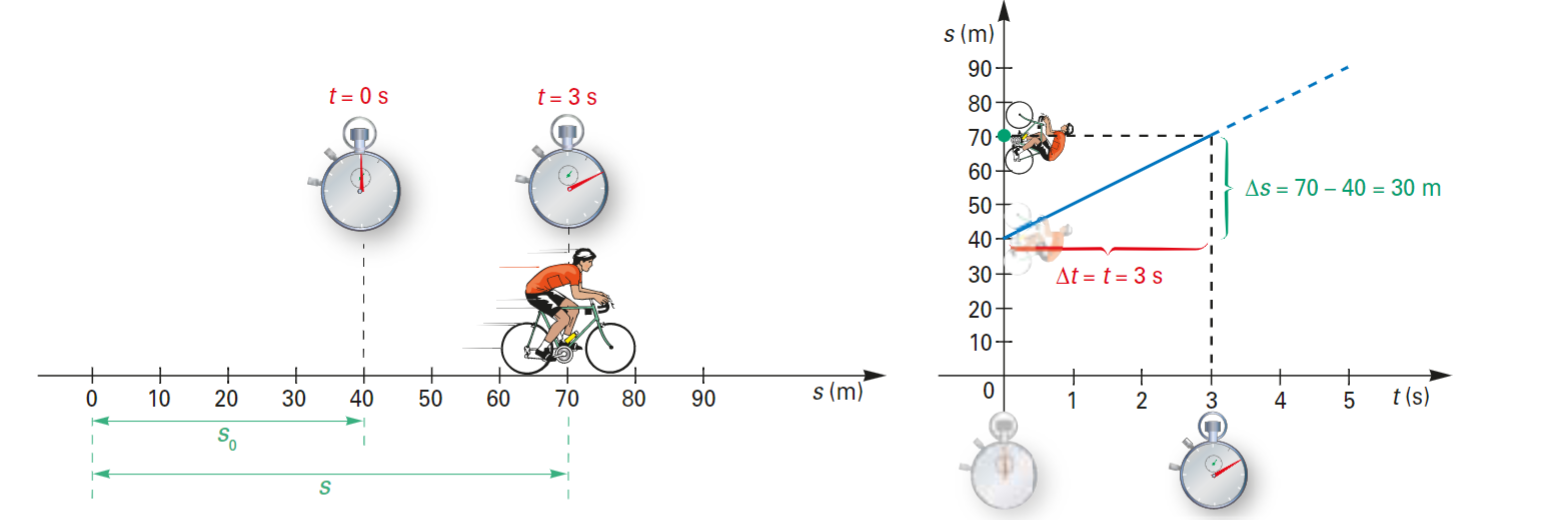
\includegraphics[scale=0.37]{moto_uniforme.png}

Il grafico spazio-tempo è una retta, non in generale passante per l'origine: l'importante è che presi due punti qualsiasi la pendenza, cioè la velocità sia costante.



\end{frame}


\begin{frame}
\frametitle{La legge oraria per il moto uniforme}

\begin{wrapfloat}{figure}{I}{0pt}
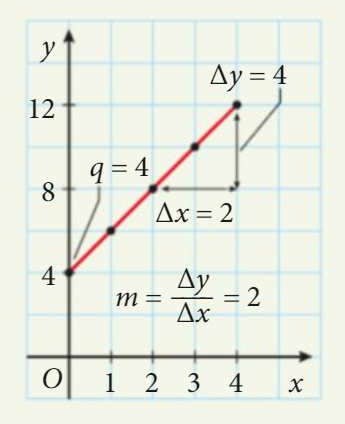
\includegraphics[width=0.5\columnwidth]{dipendenza_lineare.png}
\end{wrapfloat}

La dipendenza della coordinata spaziale da quella indipendente, temporale rispecchia la \emph{dipendenza lineare}: una funzione dl genere, nel piano cartesiano ha equazione

$
y(x) = q + m x
$

Per questo possiamo dedurre la \emph{legge oraria del moto uniforme} dal grafico spazio-tempo:
$
s(t) = s_0 + v t
$
Che esprime la dipendenza lineare dello spazio dal tempo attraverso la velocità.

\end{frame}


\begin{frame}
\frametitle{Il grafico velocità-tempo}
Un utile strumento per visualizzare la variazione del tempo della velocità di un punto materiale è il \emph{grafico velocità-tempo} 
Ad esempio per il moto uniforme corrisponde al grafico di una retta orizzontale, cioè una funzione costante: 
$ v(t) = v_0 $ 

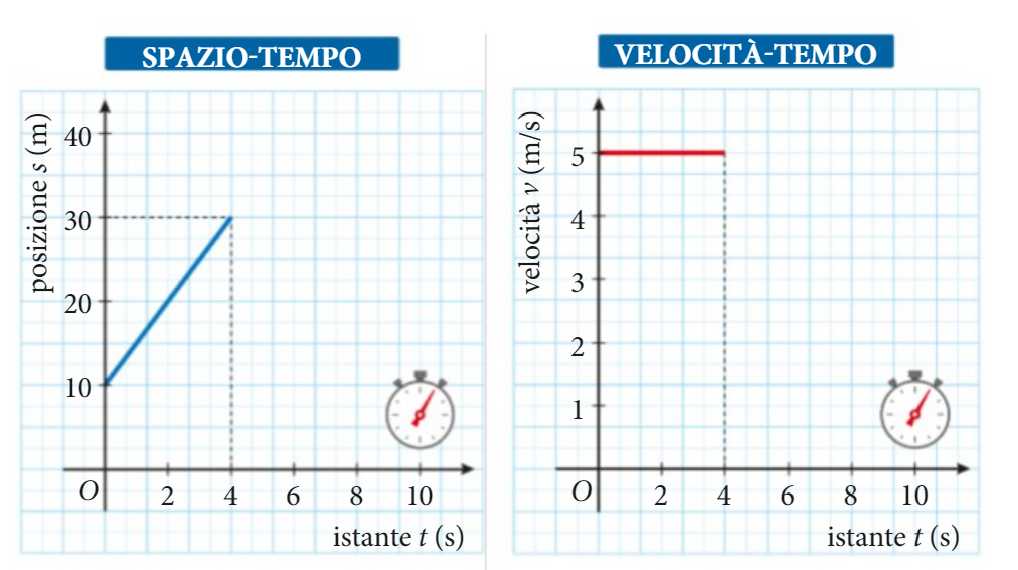
\includegraphics[scale=0.6]{spazio_velocità_tempo.png}

\end{frame}


\begin{frame}
\frametitle{Il calcolo dello spazio percorso dal grafico v-t}

Nel caso in cui $s_0 = 0$, la legge oraria si scrive semplicemente $s(t) = v t$ e lo spazio percorso può essere calcolato a partire dal grafico sotto la curva, cioè come l'area del rettangolo

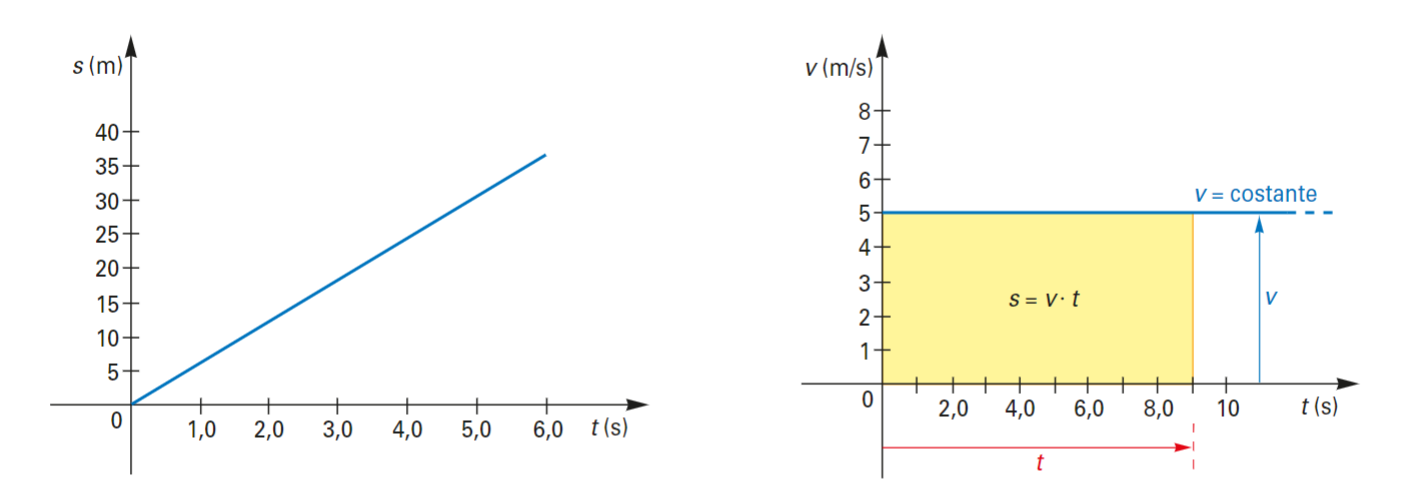
\includegraphics[scale=0.4]{spazio_percorso_v_t.png}
\[
s(t_1) = s_0 + v t_1 = 0 + v_0 t_1 = area \ \  del  \ \ rettangolo
\]

\end{frame}


\begin{frame}
\frametitle{L'accelerazione}
Poniamo il caso di studiare il moto di un punto materiale la cui velocità varia col tempo. Dato che la velocità è un vettore, come lo spostamento, allora potrebbe anche capitare, come nel moto di una particella su un'orbita circolare, che sia presente una variazione solo nella direzione. In quest'ultimo caso ed in generale quando la velocità varia, parliamo di un moto accelerato.

\begin{definizione}
Si definisce accelerazione media il rapporto tra la variazione della velocità nel tempo min cui essa avviene
\end{definizione}
\[
a_m = \frac{\Delta v}{\Delta t} = \frac{v_f - v_i}{t_f - t_i}
\]
Dove abbiamo considerato il moto unidimensionale, e quindi non abbiamo bisogno di considerare la velocità come vettore.

\end{frame}


\begin{frame}
\frametitle{L'accelerazione media nel grafico v-t}

\begin{wrapfloat}{figure}{I}{0pt}
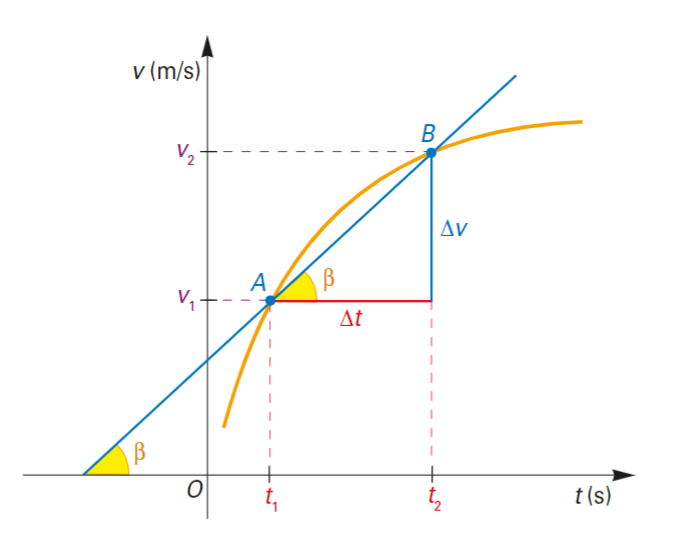
\includegraphics[width=0.5\columnwidth]{accelerazione_media_v_t.png}
\end{wrapfloat}

Come nel grafico spazio-tempo la pendenza della retta secante tra due punti era la velocità media, analogamente nel grafico velocità-tempo di un moto accelerato, l'accelerazione media è individuabile come la secante in due punti del grafico


Se gli intervalli di tempo sono presi sempre più piccoli, come nel caso della velocità istantanea nel grafico s-t, ora nel grafico v-t, definiamo l'accelerazione istantanea in un punto A come il coefficiente angolare della tangente al grafico in quel punto.

\end{frame}


\begin{frame}
\frametitle{L'accelerazione istantanea}

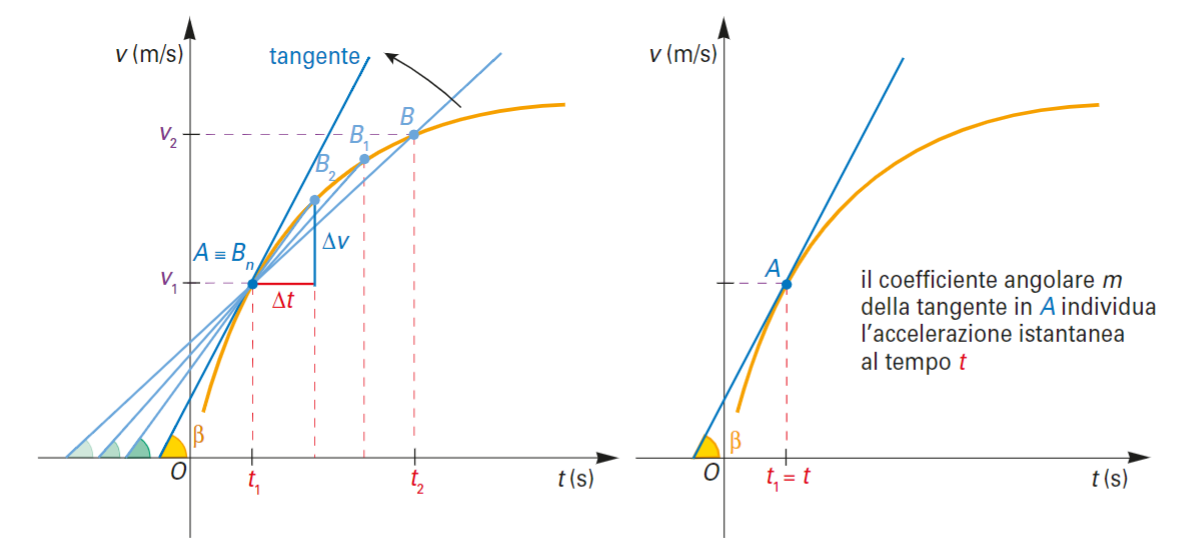
\includegraphics[scale=0.4]{accelerazione_istantanea.png}


Come abbiamo già detto, se gli intervalli vengono presi sempre più piccoli, la pendenza della secante approssima sempre meglio quella della tangente, ovvero possiamo dire che l'accelerazione istantanea è la \emph{derivata} rispetto al tempo della velocità.

\[
a = \lim\limits_{\Delta t \to 0} \frac{\Delta v}{\Delta t} \Def \frac{dv}{dt}
\]

\end{frame}


\begin{frame}
\frametitle{Il moto uniformemente accelerato}

Se in un moto con velocità variabile, accade che presi due punti qualunque del grafico v-t la pendenza è sempre costante, questo significa che l'accelerazione è costante rispetto al tempo.

\begin{definizione}
In un moto rettilineo, se l'accelerazione non varia nel tempo si parla di moto uniformemente accelerato
\end{definizione}

\begin{wrapfloat}{figure}{I}{0pt}
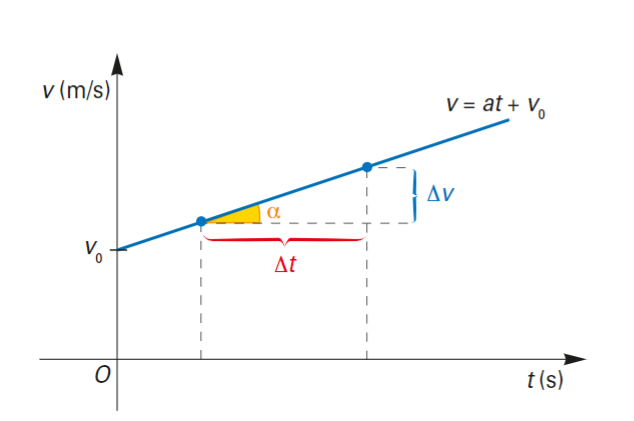
\includegraphics[width=0.5\columnwidth]{velocità_tempo_moto_uniformemente_accelerato.png}
\end{wrapfloat}

Il grafico v-t per il moto con accelerazione costante esprime la dipendenza lineare della velocità dal tempo, attraverso l'accelerazione. 

In analogia, abbiamo quindi 
$ v(t) = v_0 + a t $

con $v_0$ velocità all'istante iniziale $t_0=0$.

\end{frame}


\begin{frame}
\frametitle{Un errore molto comune \dots}

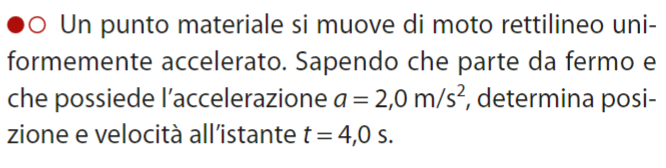
\includegraphics[scale=0.75]{prob_61_pag_42_FTE.png}

Nel problema in esame, calcoliamo la velocità finale: sfruttando la definizione di accelerazione ed invertendo la formula otteniamo, con $v_0 = 0$ 
\[
\Delta v = v - v_0 = a t = 2.0 m/s^2 \cdot 4s = 8 m/s
\]
Generalmente l'errore che si fa è quello di calcolare lo spazio percorso tramite la relazione, con $s_0 = 0$
\[
\Delta s = v t = 8 m/s \cdot 4s = 32 m
\]
Quest'errore è molto comune, ed è anche molto grave perché sfrutta la legge oraria per il moto uniforme in un caso di moto accelerato, cioè in un moto con velocità variabile nel tempo!
\end{frame}


\begin{frame}
\frametitle{Lo spazio percorso in caso di velocità variabile}

\begin{wrapfloat}{figure}{I}{0pt}
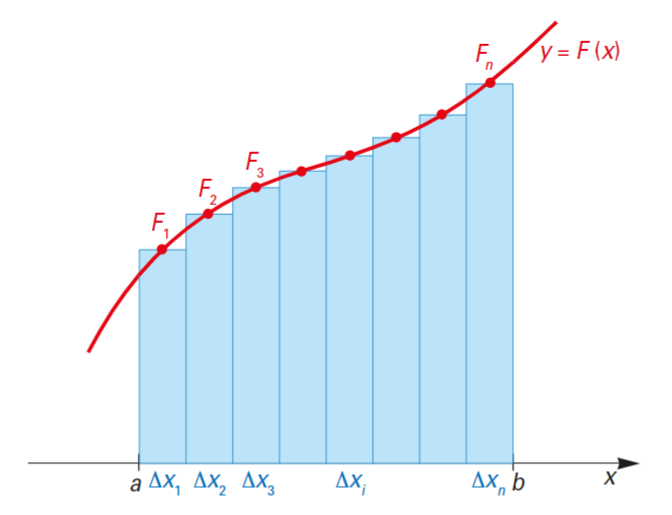
\includegraphics[width=0.5\columnwidth]{integrale_definito.png}
\end{wrapfloat}

Per risolvere il problema una soluzione potrebbe essere quella di suddividere il grafico velocità-tempo, nel caso di un moto con velocità variabile, in tanti piccoli intervalli e supporre che in ognuno si possa considerare approssimativamente la velocità costante: in questo modo $\Delta s$ si può calcolare come la somma di tutti questi piccoli spostamenti:

\[
\Delta s = v_1 \Delta t_1 + v_2 \Delta t_2 + v_3 \Delta t_3 + \dots
\]
\end{frame}


\begin{frame}
\frametitle{L'integrale definito}
In questo modo vediamo che più la suddivisione si fa fitta più lo spazio percorso uguaglia l'area sotto la curva del grafico velocità-tempo. In matematica la quantità calcolata è proprio l'\emph{integrale definito} della velocità rispetto al tempo e nel caso generale di velocità variabile avremmo: 
\[
s_f = s(t_f) = s_0 + \int_{t_0} ^{t_f} v(t) dt
\]

\begin{wrapfloat}{figure}{I}{0pt}
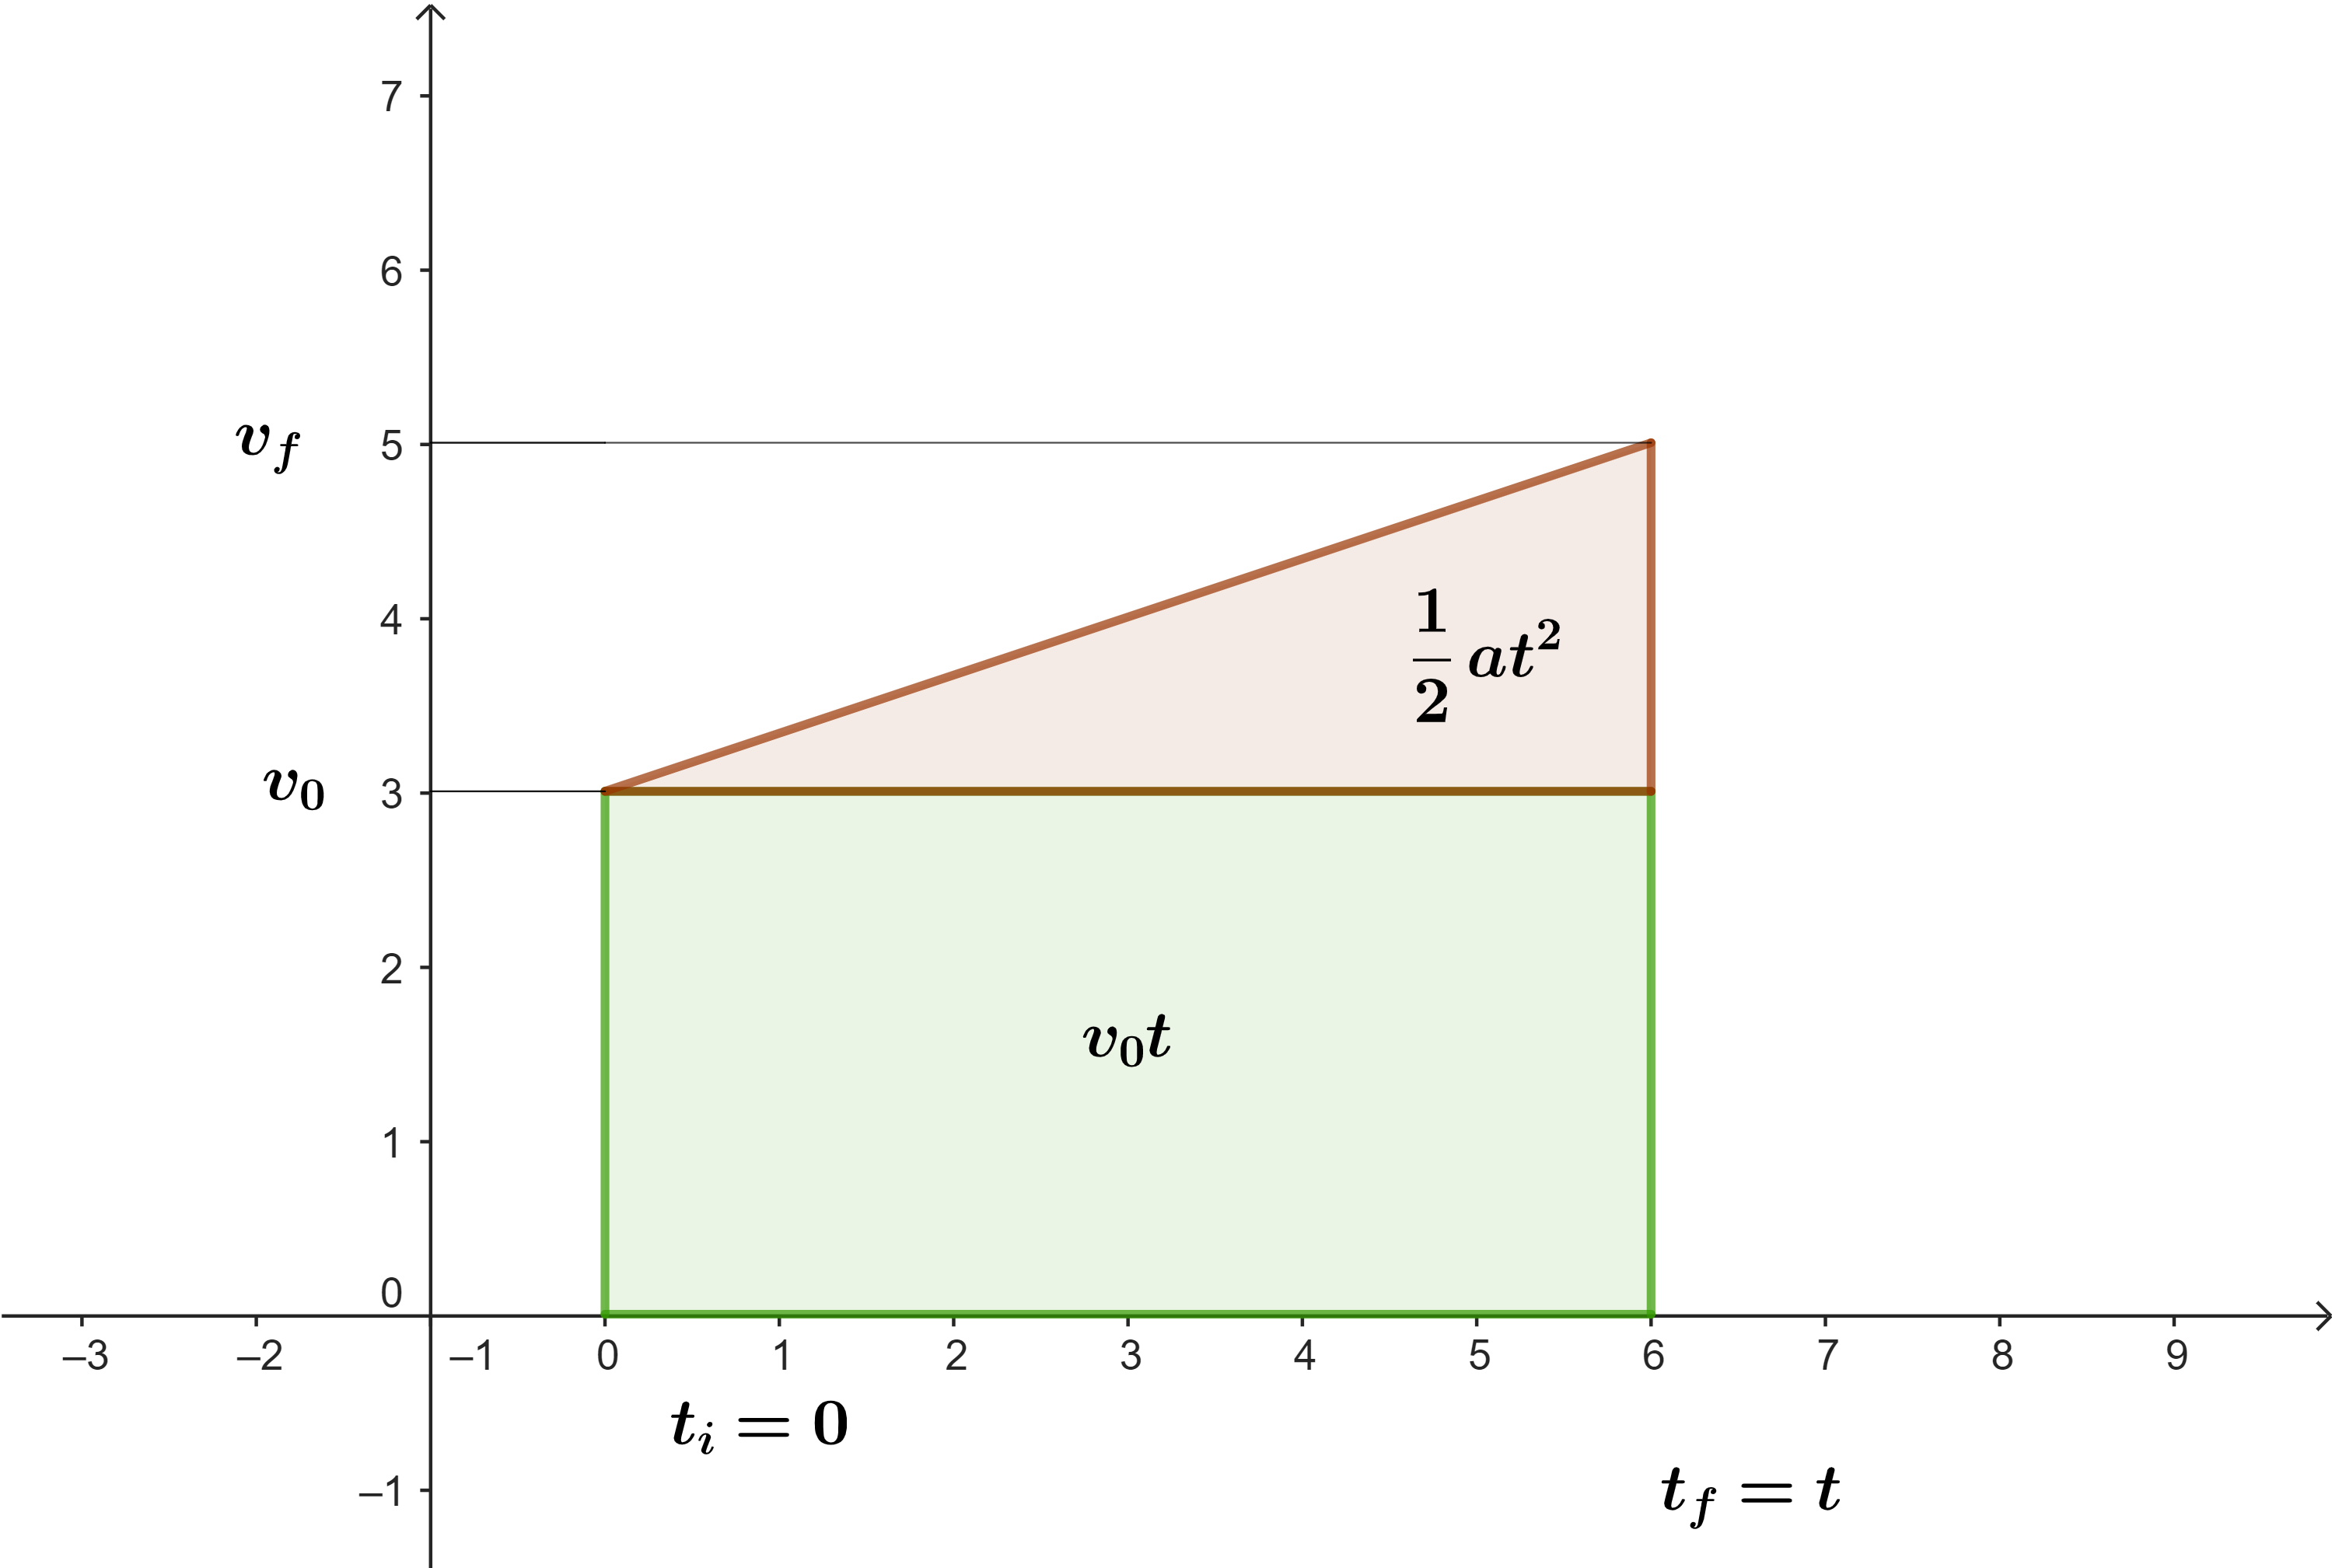
\includegraphics[width=0.5\columnwidth]{moto_uniformemente_accelerato_legge_oraria.png}
\end{wrapfloat}

Comunque nel caso del moto uniformemente accelerato i calcoli sono molto più semplici perché si può calcolare l'area sotto la curva come la somma dell'area del rettangolo più quella del triangolo

\end{frame}


\begin{frame}
\frametitle{La legge oraria per il moto uniformemente accelerato}
L'area sotto la curva si calcola quindi 
\[
\int_{t_0} ^{t_f} v(t) dt = v_0 \Delta t + \frac{(v_f - v_0)\Delta t}{2}
\]
ma $ v_f - v_0 = \Delta v = a \Delta t $ e quindi 
\[
\Delta s = v_0 \Delta t + \frac{1}{2} a (\Delta t)^2
\]
o, più semplicemente, se assumiamo $t_0 = 0$
\[
s(t) = s_0 + v_0 t + \frac{1}{2} a  t^2
\]
che è la legge oraria per il moto rettilineo uniformemente accelerato.

Possiamo usare questo risultato per completare correttamente il problema precedente ($s_0 = 0 $ e $ v_0 = 0$):
\[
s(t_f = 4s) = \frac{1}{2} a t_f ^2 = 1/2 \cdot 2 m/s^2 \cdot (4s)^2 = 16 m
\]


\end{frame}


\begin{frame}
\frametitle{Una formula utile per il moto uniformemente accelerato}

Può essere utile, per risolvere velocemente gli esercizi una formula che non coinvolga il tempo nel calcolo dello spazio percorso per il caso del moto uniformemente accelerato:

Prendiamo la legge oraria con $s_0 = 0$ e $t_0 = 0$
\[
s =  v_0 t + \frac{1}{2} a  t^2
\]
per eliminare il tempo, sfruttiamo la formula inversa della definizione di accelerazione:
$\Delta v = v_f - v_0 = a t$ e quindi $t =\frac{v_f - v_0}{a}$
Sostituendo nella legge oraria e svolgendo i calcoli abbiamo:
\[
s =  v_0 \frac{v_f - v_0}{a} + \frac{1}{2} \frac{(v_f - v_0)^2}{a} = \frac{v_f v_0}{a} - \frac{v_0 ^2}{a}  + \frac{v_f ^2}{2a}
- \frac{v_f v_0}{a} + \frac{v_0 ^2}{2a}
\]
cioè $s = \frac{v_f ^2 - v_0 ^2}{2a}$, ovvero riordinando meglio
\[
2as = v_f ^2 - v_0 ^2
\]

\end{frame}


\begin{frame}
\frametitle{Una formula utile per il moto uniformemente accelerato}
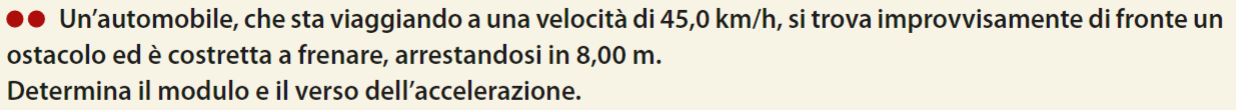
\includegraphics[scale=0.75]{es_66_pag_45_FTE.png}
Abbiamo $v_0 = 45 km/h$ e $s = 8 m$. Dato che $v_f = 0$ ed utilizzando la $2as = v_f ^2 - v_0 ^2$, abbiamo che l'accelerazione è:
\[
a = - \frac{v_0^2}{2s} =  - \frac{(45 km/h)^2}{2 \cdot 8m} = 
   - \frac{(45/3.6)^2 m^2}{16 m \cdot s^2} \approxeq -9.77 m/s^2
\]
Il segno negativo ci dice che l'accelerazione ha verso opposto al moto dell'auto, infatti l'auto sta frenando e subisce una decelerazione.   


\end{frame}


\end{document}